% This file was created with tikzplotlib v0.10.1.
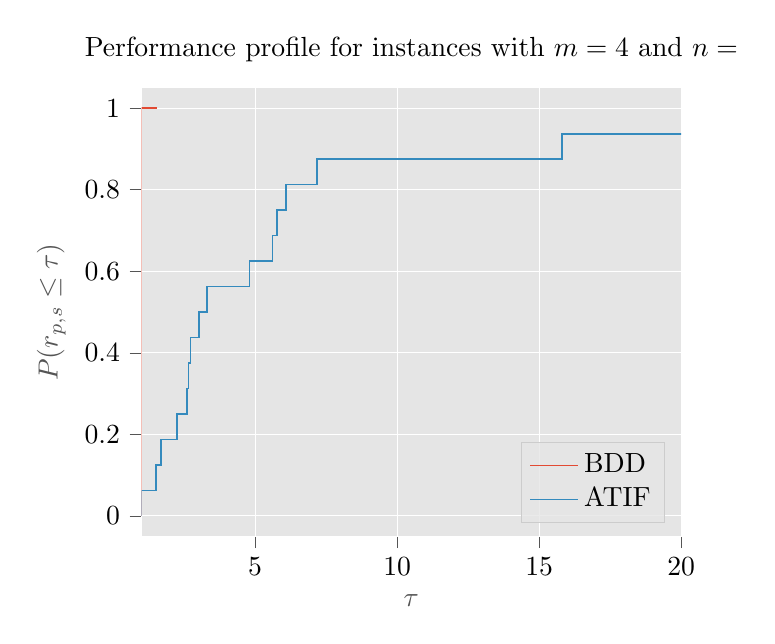
\begin{tikzpicture}

\definecolor{chocolate2267451}{RGB}{226,74,51}
\definecolor{dimgray85}{RGB}{85,85,85}
\definecolor{gainsboro229}{RGB}{229,229,229}
\definecolor{lightgray204}{RGB}{204,204,204}
\definecolor{steelblue52138189}{RGB}{52,138,189}

\begin{axis}[
axis background/.style={fill=gainsboro229},
axis line style={white},
legend cell align={left},
legend style={
  fill opacity=0.8,
  draw opacity=1,
  text opacity=1,
  at={(0.97,0.03)},
  anchor=south east,
  draw=lightgray204,
  fill=gainsboro229
},
tick align=outside,
tick pos=left,
title={Performance profile for instances with \(\displaystyle m = 4\) and \(\displaystyle n = \)},
x grid style={white},
xlabel=\textcolor{dimgray85}{\(\displaystyle \tau\)},
xmajorgrids,
xmin=1, xmax=20,
xtick style={color=dimgray85},
y grid style={white},
ylabel=\textcolor{dimgray85}{\(\displaystyle P(r_{p,s} \leq \tau)\)},
ymajorgrids,
ymin=-0.05, ymax=1.05,
ytick style={color=dimgray85}
]
\addplot [semithick, chocolate2267451, const plot mark right]
table {%
1 0
1 0.0625
1 0.125
1 0.1875
1 0.25
1 0.3125
1 0.375
1 0.4375
1 0.5
1 0.5625
1 0.625
1 0.6875
1 0.75
1 0.8125
1 0.875
1 0.9375
1.54822354246575 1
};
\addlegendentry{BDD}
\addplot [semithick, steelblue52138189, const plot mark right]
table {%
1 0
1.51130500452097 0.0625
1.68189826742641 0.125
2.25934450767471 0.1875
2.59769934050957 0.25
2.65303734715367 0.3125
2.72970284592838 0.375
3.01379533472415 0.4375
3.31584831048609 0.5
4.80387017988421 0.5625
5.61103648754132 0.625
5.76265308356947 0.6875
6.08038011364099 0.75
7.18098943485787 0.8125
15.8013789496913 0.875
291.052677077513 0.9375
326.769757564061 1
};
\addlegendentry{ATIF}
\end{axis}

\end{tikzpicture}
